% For more details: https://www.sharelatex.com/learn/Beamer

\documentclass[aspectratio=169,xcolor=dvipsnames]{beamer}					% Document class

\usepackage[english]{babel}				% Set language
\usepackage[utf8x]{inputenc}			% Set encoding
\usepackage{color}	
\usepackage{tikz}
\usepackage{amsmath}
\usepackage{amssymb}
\usepackage{bbm}
\usepackage{appendixnumberbeamer}
\usepackage[export]{adjustbox}

\newcommand{\Ell}{\mathcal{L}}
\newcommand{\mb}{\mathbf}
\newcommand{\ind}{\mathbbm{1}}
\newcommand{\E}{\mathbbm{E}}

\mode<presentation>						% Set options
{
  \usetheme{default}					% Set theme
  \usecolortheme{default} 				% Set colors
  \usefonttheme{default}  				% Set font theme
  \setbeamertemplate{caption}[numbered]	% Set caption to be numbered
  \setbeamertemplate{frametitle}[default][center]
  \beamertemplatenavigationsymbolsempty % Remove Nav Bar
  \setbeamertemplate{footline}[frame number] % Add page number in footer
  \setbeamercolor{title}{fg=black}
  \setbeamercolor{frametitle}{fg=black}
}
\usepackage{graphicx}					% For including figures
\usepackage{booktabs}					% For table rules
\usepackage{hyperref}					% For cross-referencing

\title{\hspace{0.2in}LEGEND-T2DM: Emerging Best Practices}	% Presentation title
\author{Fan Bu and Aki Nishimura}								% Presentation author
\institute{on behalf of the LEGEND initiative}					% Author affiliation
\date{October 2021}	

\begin{document}

% Title page
% This page includes the informations defined earlier including title, author/s, affiliation/s and the date
{
\usebackgroundtemplate{
\includegraphics[width=\paperwidth]{figures/OHDSI_title_background.jpg}}%
\begin{frame}[plain]
  \titlepage
\end{frame}
}

{
\usebackgroundtemplate{
\includegraphics[width=\paperwidth]{figures/OHDSI_content_slide_template.jpg}}
\begin{frame}{LEGEND-T2DM Methods Outline}
Methodological gaps in realizing LEGEND objectives:
\begin{itemize}
    \item Causal inference on survival outcomes
    \item Evidence synthesis on federated data
\end{itemize}
\end{frame}
}

{
\usebackgroundtemplate{
\includegraphics[width=\paperwidth]{figures/OHDSI_content_slide_template.jpg}}
\begin{frame}{Causal inference on survival outcomes}
	\hspace*{.03\linewidth}
	\begin{minipage}{.7\linewidth}
	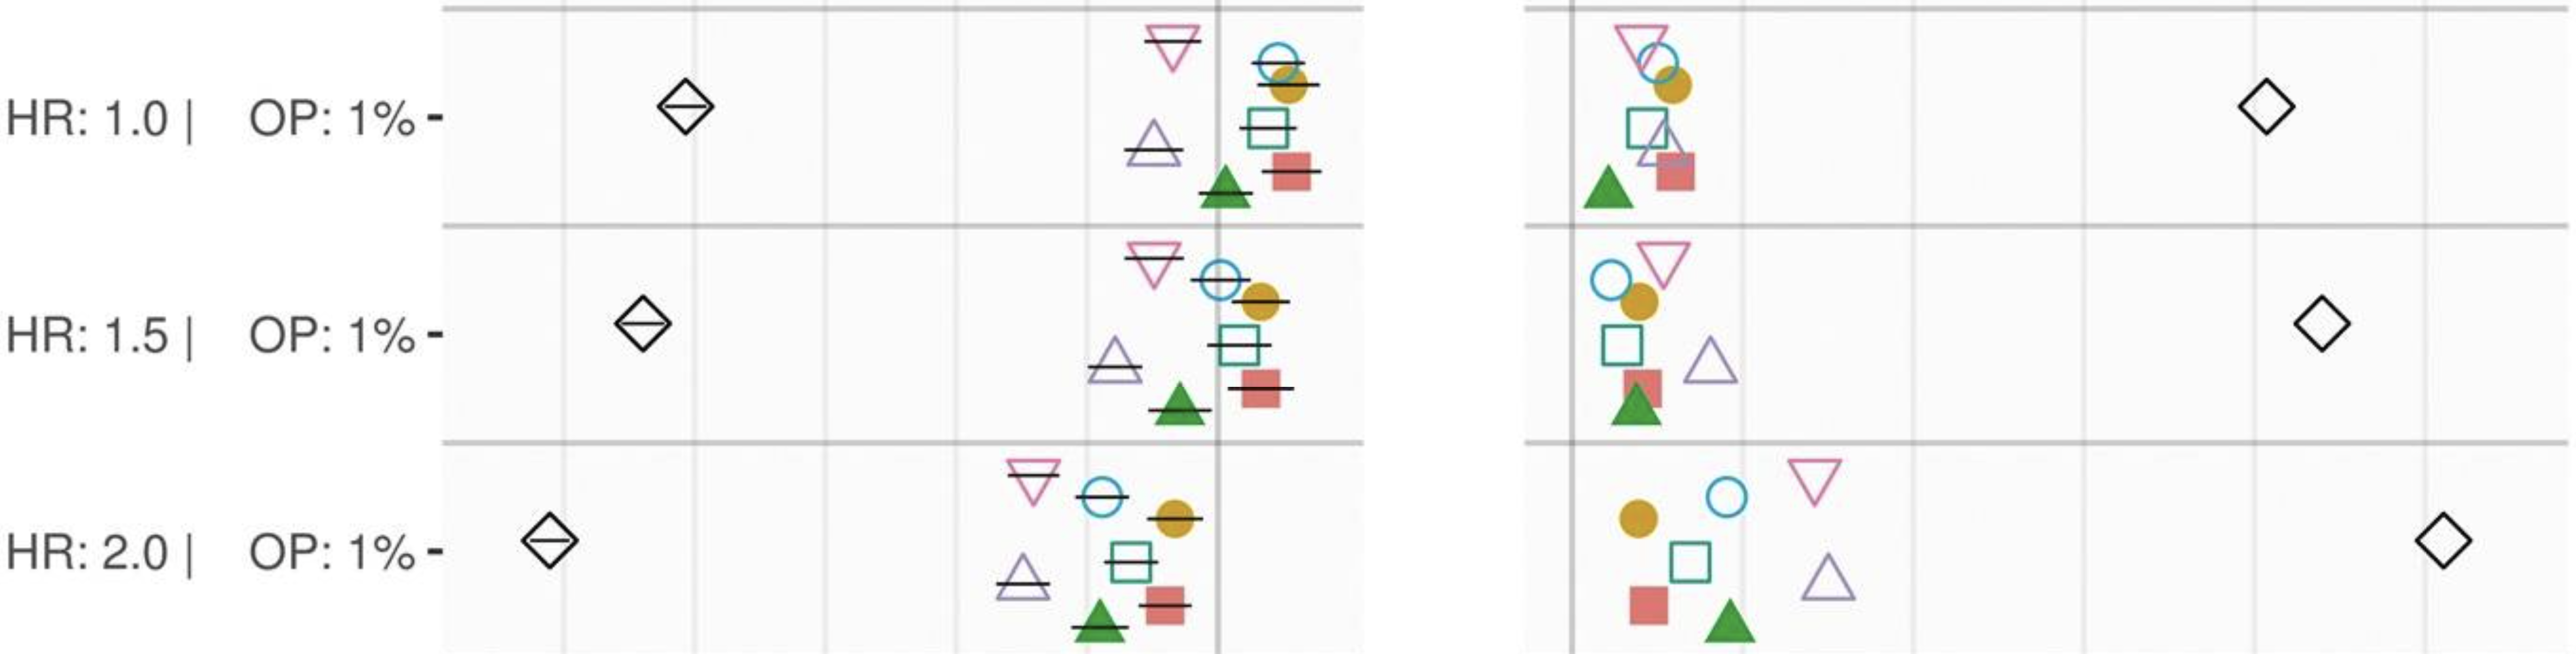
\includegraphics[width=\linewidth]{figures/positive_control_experiments_1_percent_outcome}
	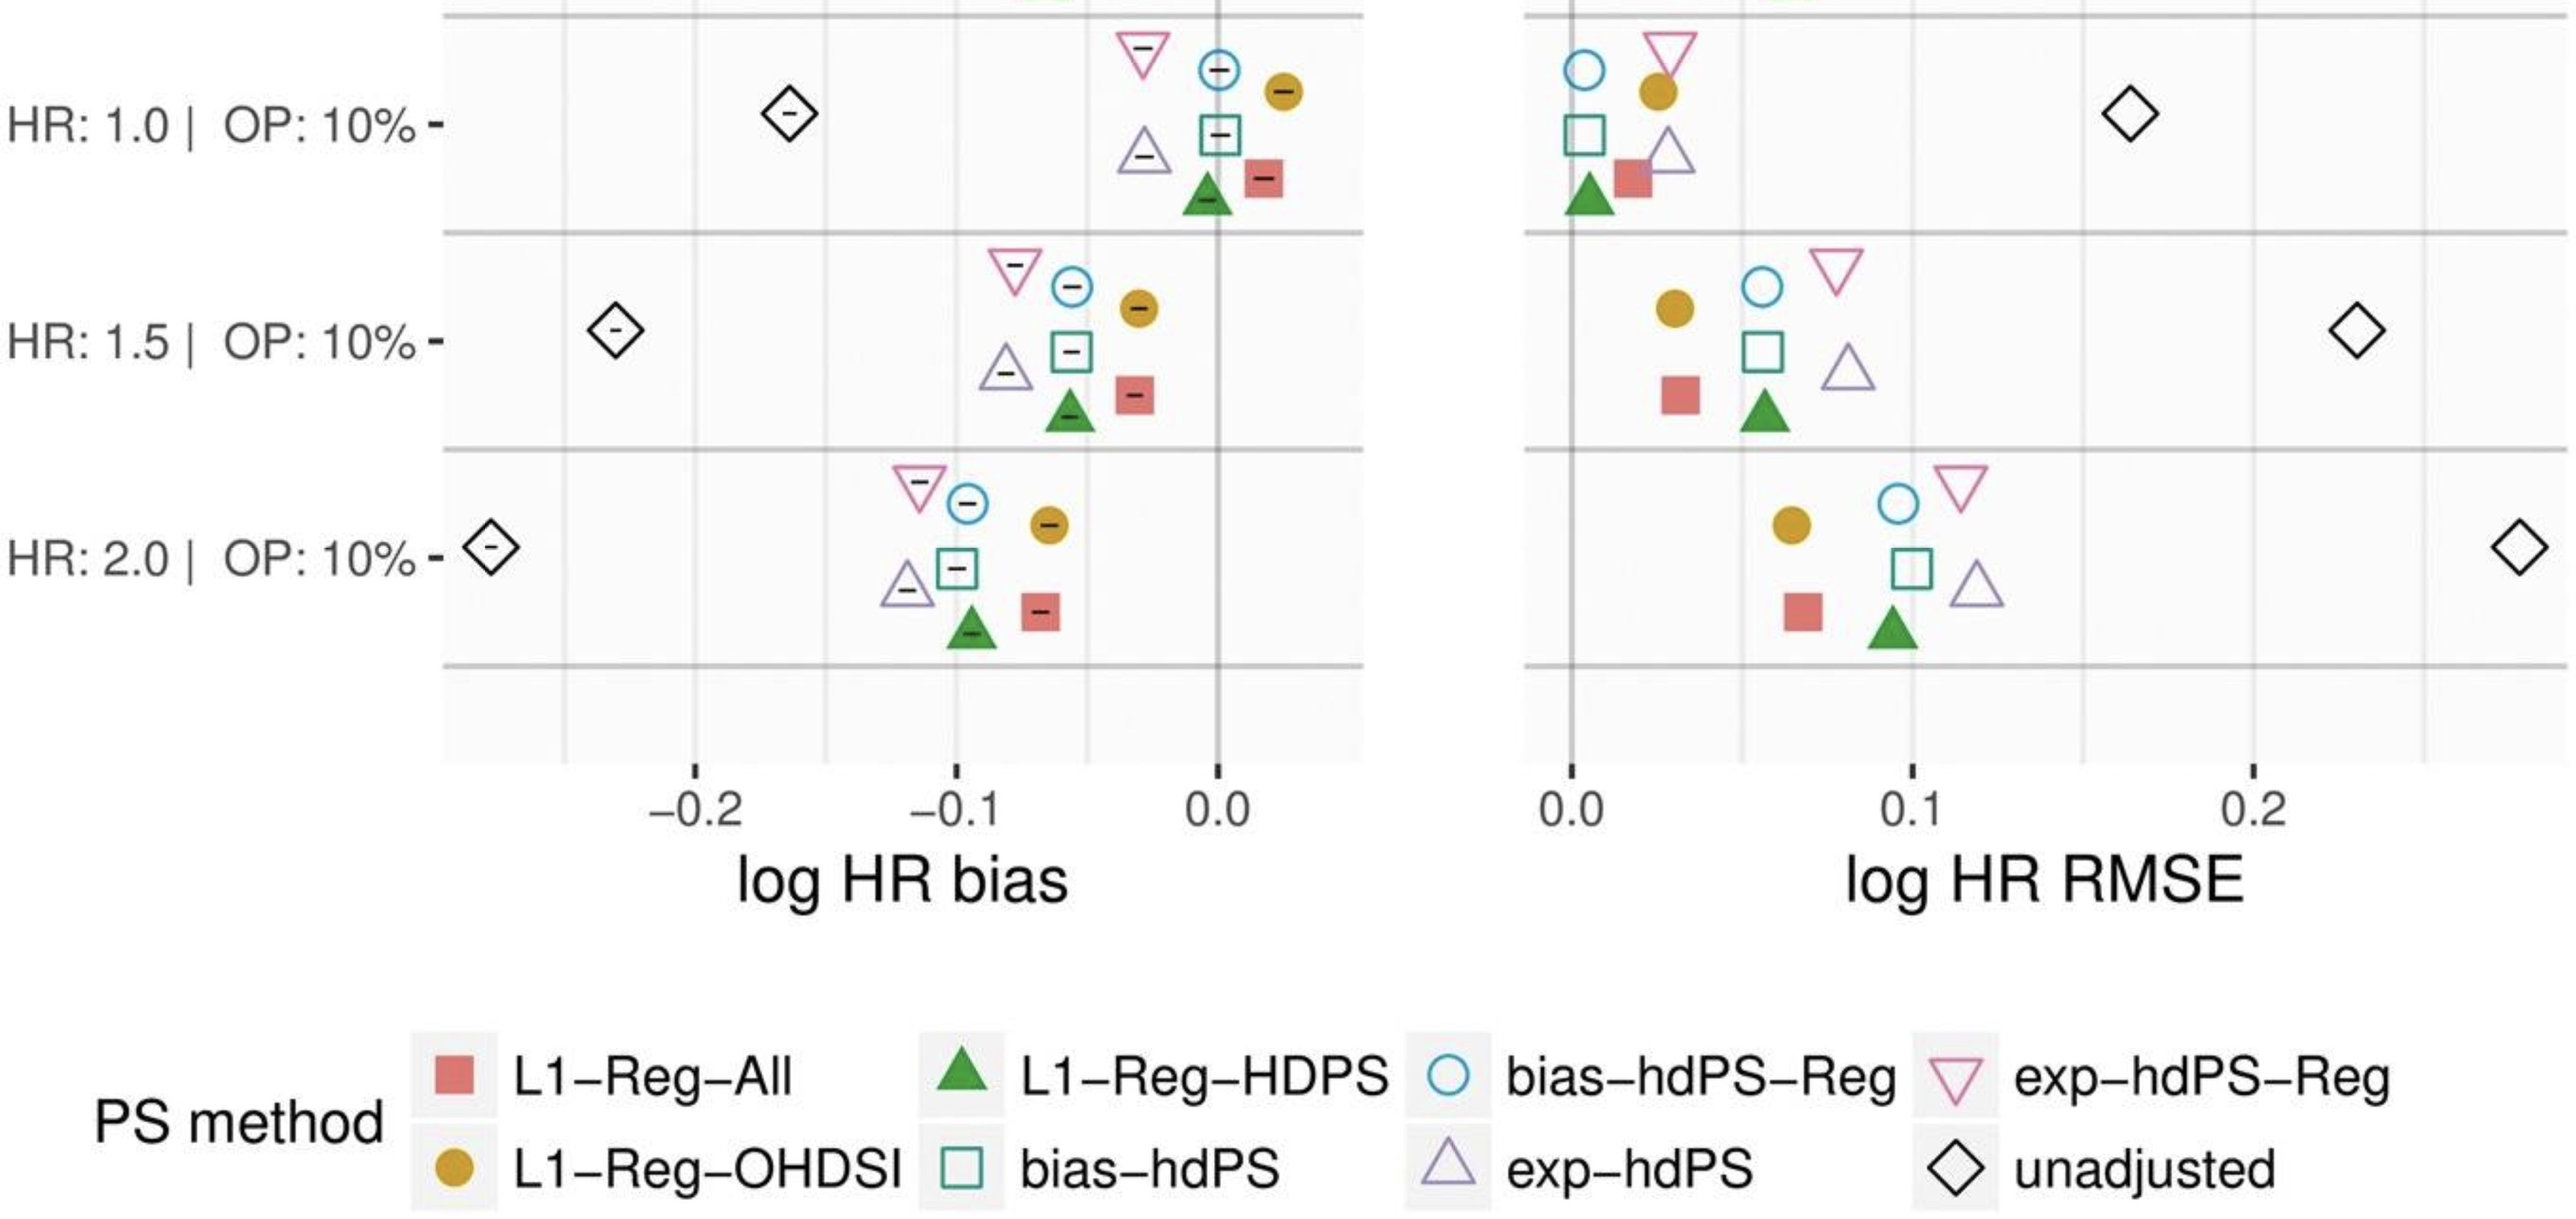
\includegraphics[width=\linewidth]{figures/positive_control_experiments_10_percent_outcome}
	\end{minipage}
	\nobreak\hspace{.15em}
	\begin{minipage}{.24\linewidth}
	Non-linearity / \\ non-collapsibility of Cox model causes \emph{bias} toward null.
	
	\pause
	\vspace*{\baselineskip}
	But only in case of sufficiently large\\ hazard ratio and/or high outcome prevalence.
	\end{minipage}
\end{frame}
}

{
\usebackgroundtemplate{
\includegraphics[width=\paperwidth]{figures/OHDSI_content_slide_template.jpg}}
\begin{frame}{Causal inference on survival outcomes}
	\begin{minipage}{\linewidth}
	\vspace*{.07\paperheight}
	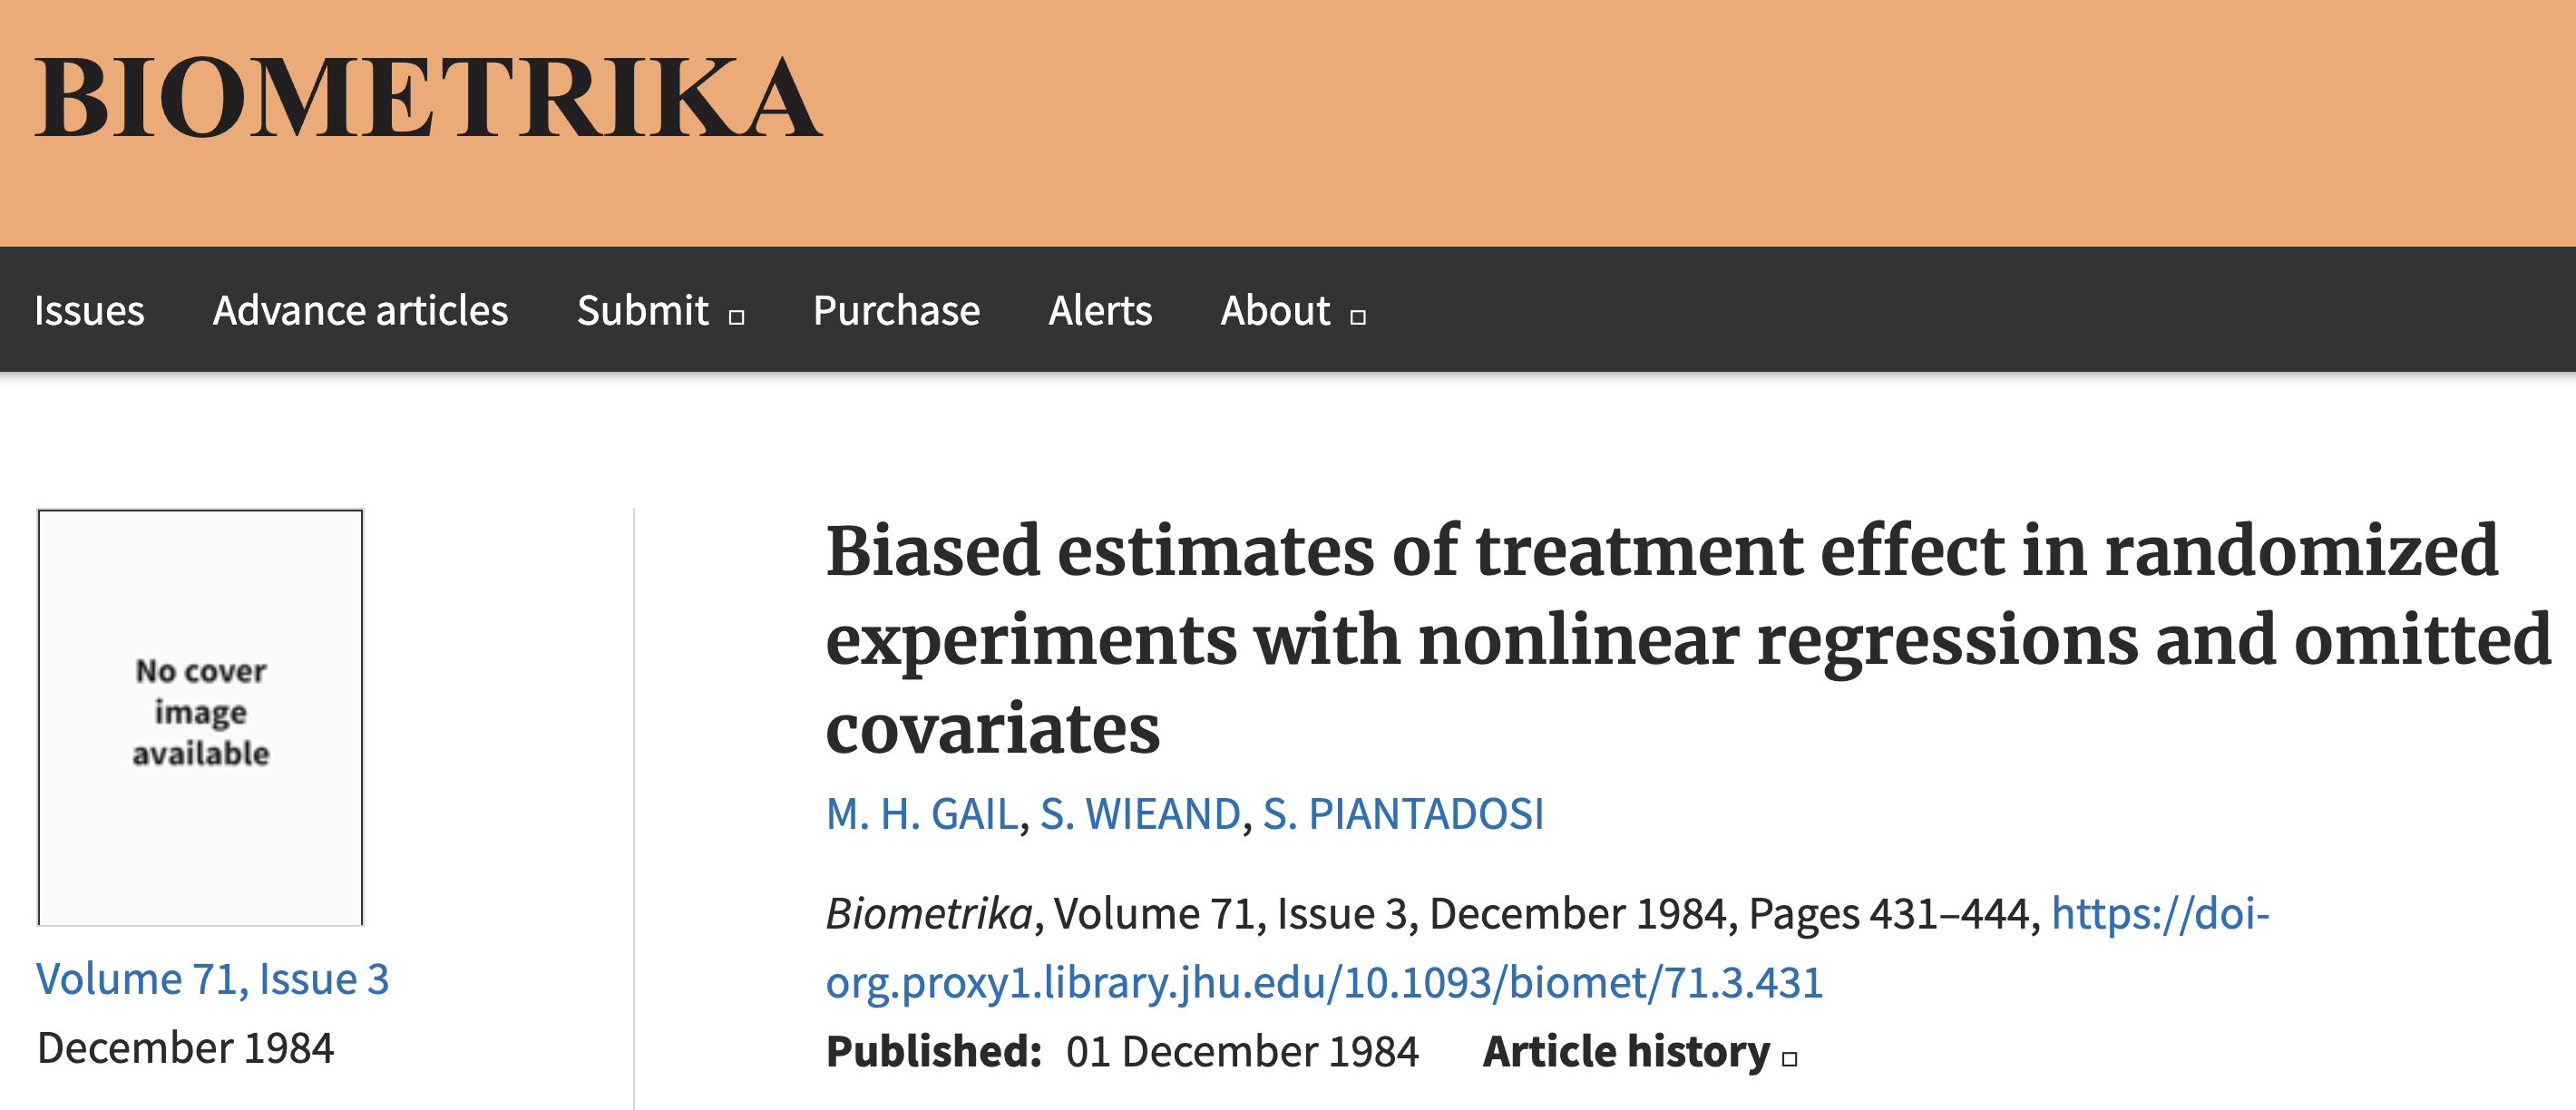
\includegraphics[width=0.6\linewidth]{figures/gail_et_al_1984}
	\end{minipage}
	\begin{minipage}{\linewidth}
	\raggedleft
	\vspace*{-.15\paperheight}
	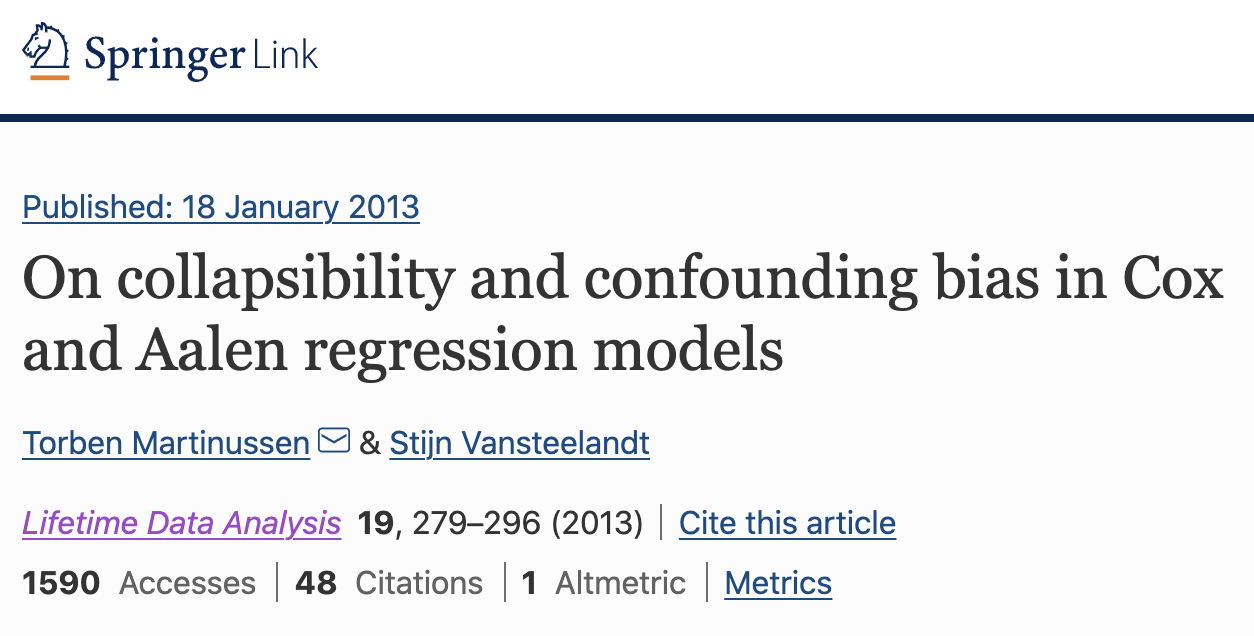
\includegraphics[width=0.45\linewidth]{figures/martinussen_vansteelandt_2013}
	\end{minipage}
	\pause
	\begin{minipage}{\linewidth}
	\centering
	\vspace*{-.6\paperheight}
	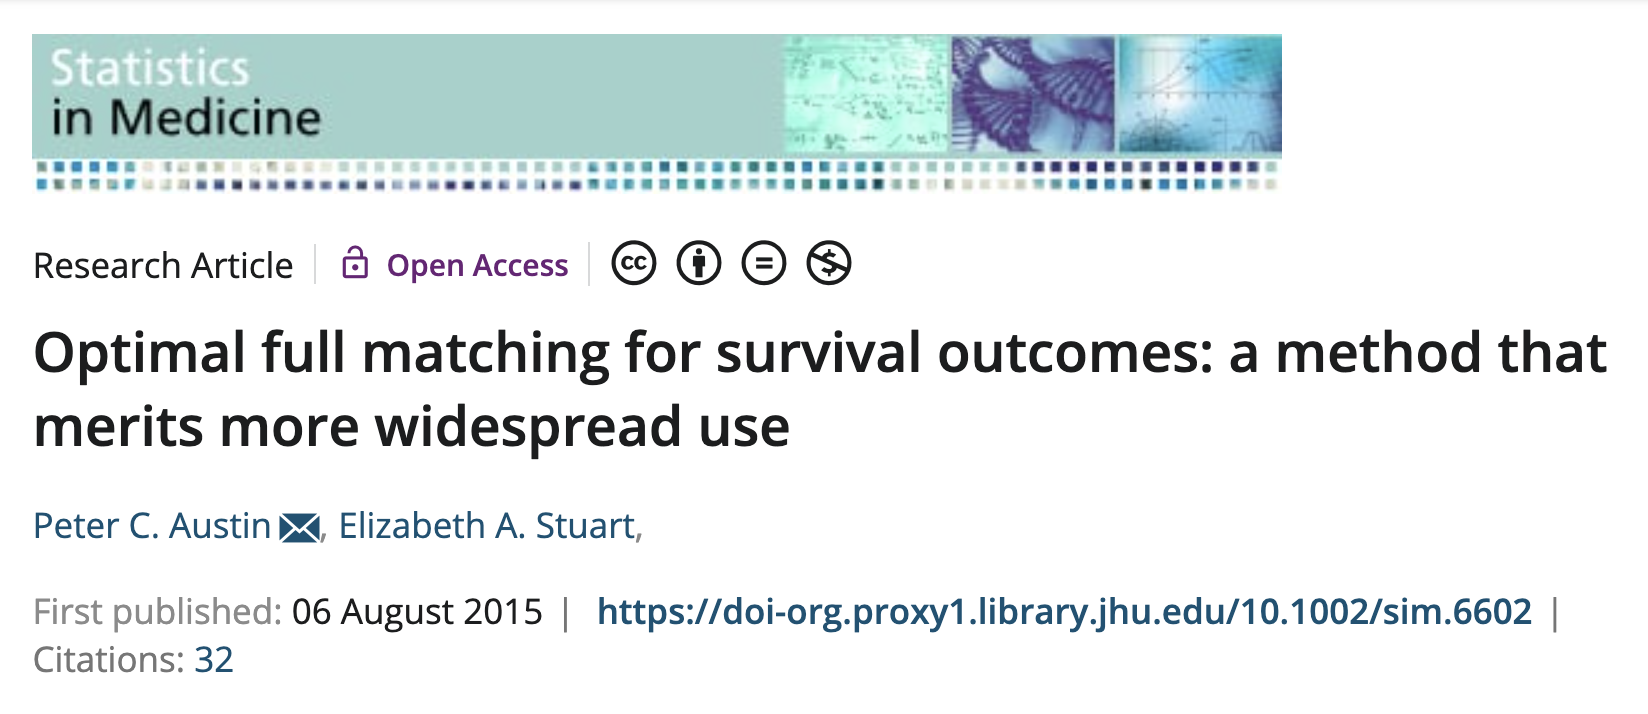
\includegraphics[width=0.55\linewidth, frame]{figures/austin_stuart_2015}
	\end{minipage}
\end{frame}
}

{
\usebackgroundtemplate{
\includegraphics[width=\paperwidth]{figures/OHDSI_content_slide_template.jpg}}
\begin{frame}{Evidence synthesis: traditional method}
\begin{columns}
\begin{column}{0.35\textwidth}
\begin{itemize}
    \item Each site produces point estimate for effect size
    \item Use meta analysis (e.g., random effect model) to combine estimates
    \item End result is an overall estimate
\end{itemize}

\end{column}
\begin{column}{0.65\textwidth}
\begin{figure}
    \centering
    \hspace*{-0.15in}
    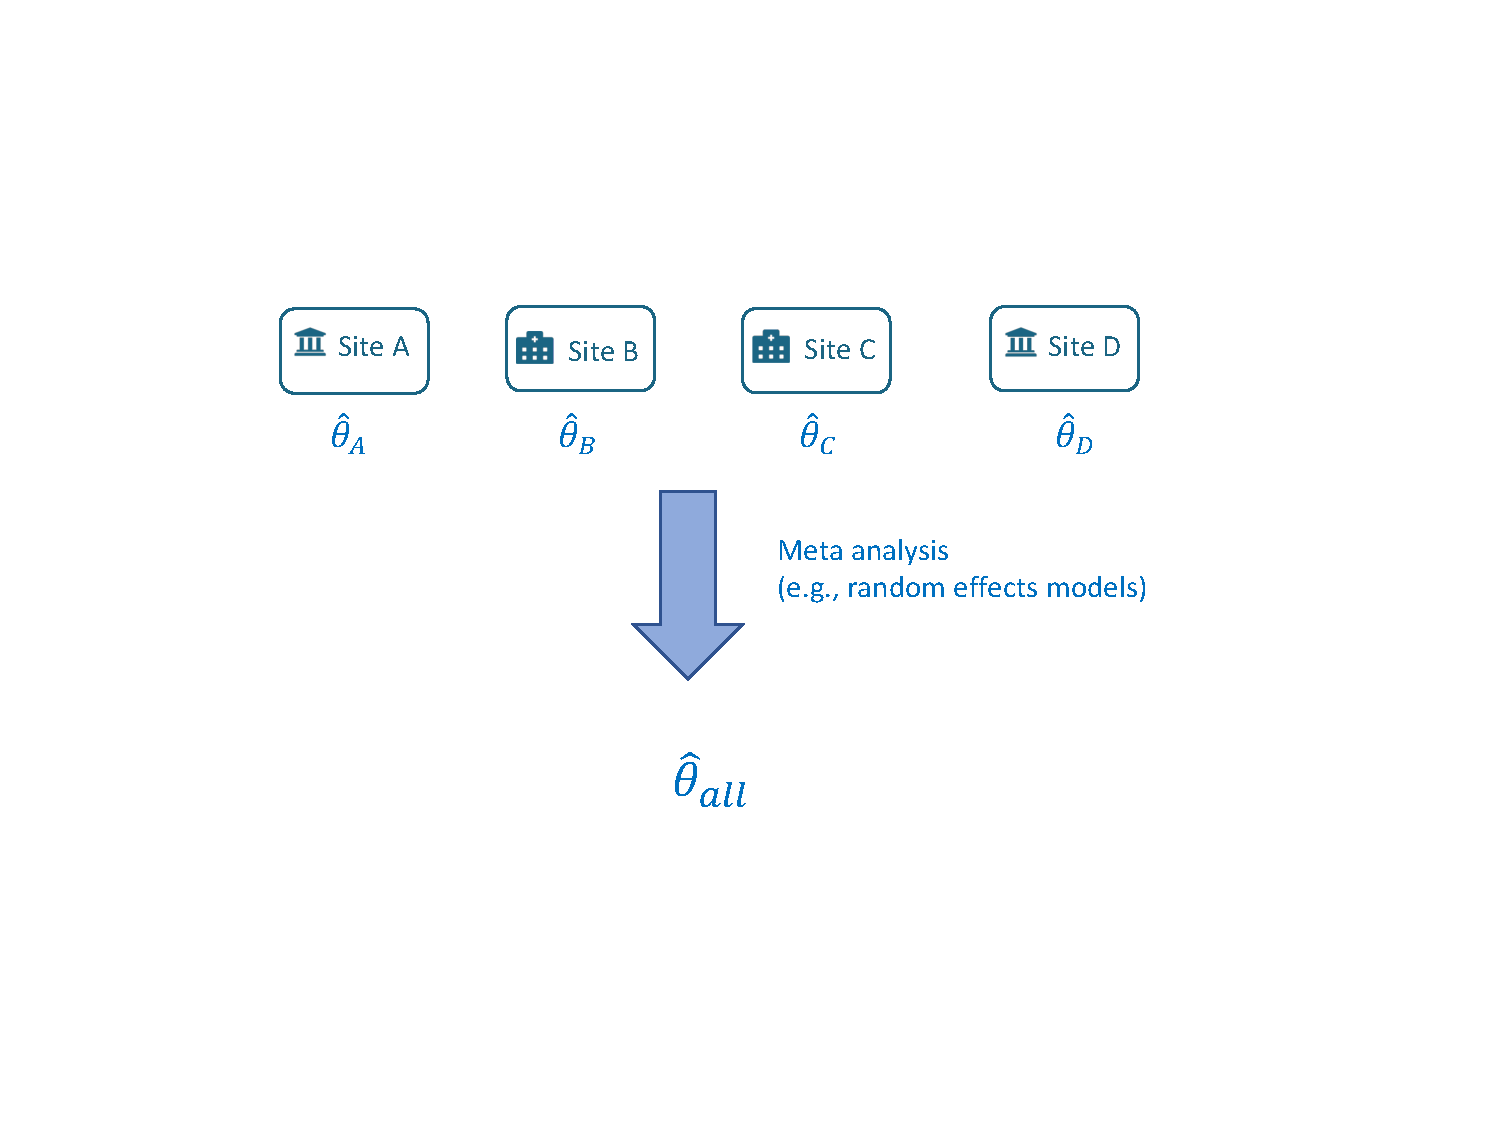
\includegraphics[trim = 0.5in 1in 0.5in 1.2in, clip, width=1.2\textwidth,page=1]{figures/Legend_hightlight_method_graphs.pdf}
    %\caption{Caption}
    %\label{fig:my_label}
\end{figure}
\end{column}
\end{columns}


\end{frame}
}


{
\usebackgroundtemplate{
\includegraphics[width=\paperwidth]{figures/OHDSI_content_slide_template.jpg}}
\begin{frame}{Evidence synthesis: emerging alternative}
\begin{columns}
\begin{column}{0.45\textwidth}
\begin{itemize}
    \item Instead...
    \item Each site produces a likelihood
    \item Likelihood: profile of full evidence
    \item Use Bayesian or numerical methods to "combine" likelihoods
    \item End result is an overall likelihood profile
\end{itemize}

\end{column}
\begin{column}{0.6\textwidth}

\begin{figure}
    \centering
    \hspace*{-0.23in}
    \includegraphics[trim = 0.5in 1in 0.5in 1.2in, clip, width=1.2\textwidth, page=2]{figures/Legend_hightlight_method_graphs.pdf}
    %\caption{Caption}
    %\label{fig:my_label}
\end{figure}
\end{column}

\end{columns}

\end{frame}
}

{
\usebackgroundtemplate{
\includegraphics[width=\paperwidth]{figures/OHDSI_content_slide_template.jpg}}
\begin{frame}{Challenges and emerging \& future work}
\begin{itemize}
    \item Small or zero counts (monotonous individual likelihoods)
    \begin{itemize}
        \item[-] need better likelihood approximations or better combination algorithms (e.g., Schuemie et al., 2021; Duan et al., 2020)
    \end{itemize}
    \item Systematic errors (common in observational data)
    \begin{itemize}
        \item[-] calibration using negative (\& positive) controls (e.g., Mulgrave et al., 2020) 
    \end{itemize}
    \item Community-level confounding
    \begin{itemize}
        \item[-] possible solution with mixture models or latent factor models 
    \end{itemize}
\end{itemize}

\end{frame}
}




\end{document}
